\documentclass{beamer}
\usepackage{beamerthemesplit,graphicx,wrapfig, slashed, verbatim,hyperref,color,colortbl,tabularx}
% \usepackage{graphicx,wrapfig, slashed, subfigure,verbatim,hyperref,color,colortbl,tabularx}
\usepackage{amsmath,amssymb}
\usepackage{helvet} %font helvetica
\usepackage{units}
\usepackage{pdftricks}
\usepackage{pstricks}
\usepackage{beamerfoils}
%\usepackage{babel}
\usepackage[utf8]{inputenc}
\usepackage[T1]{fontenc}
\usepackage{ulem}
\usepackage{epstopdf}
\usepackage{color}
\usepackage{feynmf}
\usepackage{subcaption}
%\usepackage{biblatex}
\usepackage[
  locale=DE,
  separate-uncertainty=true,
  decimalsymbol=.,
  per-mode=symbol-or-fraction,
]{siunitx}
\usepackage{multirow}

% \usetheme{Hannover}
\useoutertheme{infolines2}
%\font\ttfAkkuratLightOffice AkkuratLightOffice-Regular at10pt
\colorlet{structure}{green!50!black}
\definecolor{tugreen}{RGB}{132,184,24}
\definecolor{tugrey}{RGB}{178,179,182}
\definecolor{tured}{RGB}{205,0,47}
\setbeamercolor{palette primary}{bg=tugreen,fg=black}
\setbeamercolor{palette secondary}{bg=tugrey!50!tugreen,fg=black}
\setbeamercolor{palette quaternary}{fg=black, bg=tugrey}
\setbeamercolor{caption name}{fg=tugreen}
\setbeamercolor{palette tertiary}{fg=black,bg=tugrey}


\setbeamercolor{palette compare}{bg=white!80!tugreen,fg=black}
\setbeamercolor{palette misc}{bg=white!80!tugreen,fg=black}
\setbeamercolor{palette white}{bg=white!99!black,fg=black}

\setbeamercolor{itemize item}{fg=tugreen}
\setbeamercolor{itemize subitem}{fg=tugreen}
\setbeamercolor{itemize subsubitem}{fg=tugreen}
\setbeamercolor{enumerate item}{fg=tugreen}
\setbeamertemplate{itemize item}[square]
\setbeamercolor{titlelike}{fg=tugreen, bg=white}


\title{Studies on interference effects of flavor changing neutral currents in the top sector ($tu\gamma$,$tc\gamma$ couplings)}


\author{Salvatore La Cagnina}
\institute[TU Dortmund]{
\scriptsize Technische Universität Dortmund, Lehrstuhl EIV \\ 
\vspace{0.5cm}
}


\date{\today}

\MyLogo{
\includegraphics[width=3cm]{images/tud_logo_cmyk.pdf}} 
\setbeamertemplate{navigation symbols}{}


\begin{document}

\frame{\titlepage}

%\section{SECTION}
%\subsection{SUBSECTION}
%%\LogoOff
%\begin{frame}[fragile]
%\frametitle{FRAMETITLE}
%\begin{beamercolorbox}[rounded=true,shadow=true]{palette misc}
%	One type of colorbox
%\end{beamercolorbox}
%\begin{beamercolorbox}[rounded=true,shadow=true]{palette quaternary}
%	Second type of colorbox
%\end{beamercolorbox}
%\end{frame}




\section{General}
\subsection{Structure}
\begin{frame}[fragile]
\frametitle{Content}
%\begin{beamercolorbox}[rounded=true,shadow=true]{palette misc}
	\begin{itemize}
		\item Flavor changing neutral currents
		\item Production and decay channel
		\item Brief (current) outline of the thesis
		\item First steps
		\item Following steps
	\end{itemize}
%\end{beamercolorbox}
\end{frame}


\section{Flavour Changing}
\subsection{Neutral Current}
\begin{frame}[fragile]
\frametitle{FCNCs ($tu\gamma$-Vertex)}
\vspace{-3mm}
\begin{minipage}{0.48\textwidth}
	\begin{figure}
		\centering
		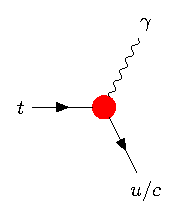
\includegraphics[width=0.6\linewidth]{images/tug-vertex.pdf}
	\caption{FCNC Vertex, changing the top quark flavor with a photon to another up type quark.}
	\end{figure}
\end{minipage}
\hfill
\begin{minipage}{0.48\textwidth}
	\begin{beamercolorbox}[rounded=true,shadow=true]{palette misc}
		\begin{itemize}
			\item Forbidden processes in the SM due to flavor conservation in QED/QCD and neutral current weak interactions 
			\item FCNCs as possible extension of the SM
			\item Supported by several theories such as 
			effective field theories etc.
		\end{itemize}
	\end{beamercolorbox}
\end{minipage}

\end{frame}

\LogoOff
\begin{frame}[fragile]
\frametitle{Production and decay channels}
\begin{minipage}{0.60\textwidth}
	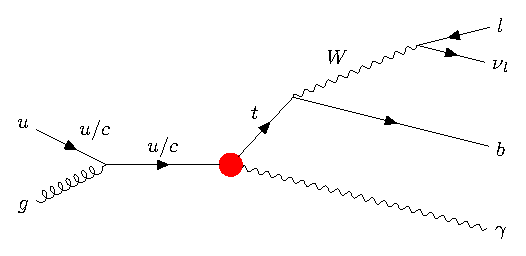
\includegraphics[width=1\linewidth]{images/prod.pdf}\\
	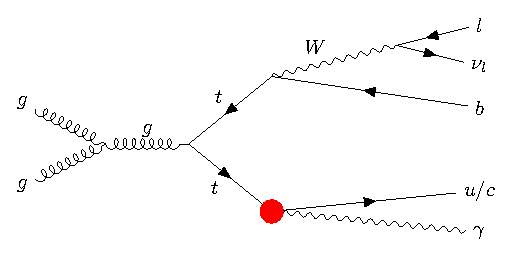
\includegraphics[width=1\linewidth]{images/decay.pdf}
\end{minipage}
\begin{minipage}{0.36\textwidth}
\vspace{-5mm}
\begin{beamercolorbox}[rounded=true,shadow=true]{palette misc}
			Separation of two different modes for the FCNC process with $tu\gamma$-Vertex
			\\
		\begin{itemize}
			\item Production Channel\\ (on top)
			\vspace{5mm}
			\item Decay Channel \\ (on bottom)
			\vspace{5mm}
			\item Main difference:\\ one additional light quark jet in decay channel
		\end{itemize}
	\end{beamercolorbox}
\end{minipage}
\end{frame}

\section{Thesis}
\subsection{Focus}

\begin{frame}[fragile]
\frametitle{Interference}
\begin{beamercolorbox}[rounded=true,shadow=true]{palette misc}
	\begin{itemize}
		\item Until now production and decay mode are shown in LO
		\item Including NLO interference between the diagrams can occur
		\item Possible influence in several distributions
		\item Search for interference as a search for FCNC
	\end{itemize}
\end{beamercolorbox}
\end{frame}

\begin{frame}[fragile]
\frametitle{First (comlpeted) steps}
\begin{beamercolorbox}[rounded=true,shadow=true]{palette misc}
	\begin{itemize}
		\item Set up MadGraph, Pythia and a basic detector simulation (DELPHES)
		\item This is done standalone without ATLAS internal software to keep it more general
		\item First generated processes ($pp \rightarrow t\bar{t} \rightarrow l^+ l^{'^{-}} \bar{\nu_{l}} \nu_{l^{'}} b \bar{b}$)
		\item First completed showering and detector simulation runs
		\item Plots are following
	\end{itemize}
\end{beamercolorbox}
\end{frame}

\begin{frame}[fragile]
\frametitle{First Plot}
Hier sollte ein hoffentlich krasser Plot sein :)
\end{frame}

\begin{frame}[fragile]
\frametitle{Next steps}
\begin{beamercolorbox}[rounded=true,shadow=true]{palette misc}
	\begin{itemize}
		\item MadGraph NLO testing
		\item Include UFO model (TopFCNC) for FCNC processes
		\item Reproduce production and decay channel analysis
		\item Get samples with both processes in NLO and hope MadGraph calculates possible interference
		\item Hope for progress and quick update, thanks for your attention
	\end{itemize}
\end{beamercolorbox}
\end{frame}

\end{document}

% \appendix
% \backupbegin
% \section{Appendix}
% \subsection{}

% \begin{frame}
% \frametitle{Observables}
% 	\begin{figure}
% 		\centering
% 		\includegraphics[width=0.8\textwidth,page=1]{plots/observables.pdf}
% 	\end{figure}
% \end{frame}

% \LogoOff
% \begin{frame}
% \frametitle{Single top measurement correlation}
% 	\begin{figure}
% 		\centering
% 		\includegraphics[width=0.7\textwidth]{plots/singletopcorrres.png}
% 	\end{figure}
% \end{frame}
% \LogoOn
%\backupend

% \newcommand{\backupbegin}{
%    \newcounter{framenumberappendix}
%    \setcounter{framenumberappendix}{\value{framenumber}}
% }
% \newcommand{\backupend}{
%    \addtocounter{framenumberappendix}{-\value{framenumber}}
%    \addtocounter{framenumber}{\value{framenumberappendix}} 
% }




%\begin{frame}
%	\frametitle{Topics} \vspace{-3mm}
%	\begin{beamercolorbox}[rounded=true,shadow=true]{palette misc}
%		\begin{itemize}
%			\item Main objective: calculate a pdf for the top quark width
%			\item Build a model with observables, measurements and parameters
%			\item Implement dependencies of the observables from the parameters
%			\item Include measurements
%			\item EFTfitter is used in order to implement that model and perform the calculation
%		\end{itemize}\vspace{2mm}
%	\end{beamercolorbox}
%\end{frame}
% \begin{frame}
% 	\frametitle{Content} \vspace{-3mm}
% 	\begin{beamercolorbox}[rounded=true,shadow=true]{palette misc}
% 		\begin{itemize}
% 			\item The Standard Model
% 			\item Top quark measurements at LHC
% 			\item Inference of model parameters in Bayesian analysis
% 			\item Implementation of Bayesian analysis in EFTfitter
% 			\item Combination of measurements with the BLUE method and the EFTfitter 
% 			\item Constraining the top quark width using EFTfitter
% 			\item Conclusion and Outlook
% 		\end{itemize}\vspace{2mm}
% 	\end{beamercolorbox}
% \end{frame}

% \section{Standard}
% \subsection{Model}
% \begin{frame}
% 	\frametitle{The Standard Model} \vspace{-3mm}
% 	\input{tables/sm.tex}
% 	\begin{beamercolorbox}[rounded=true,shadow=true]{palette misc}
% 		\begin{itemize}
% 			\item Vector bosons as mediators of fundamental forces
% 			\item Fermion mass increases per generation
% 			\item Gravitation is not included
% 		\end{itemize} \vspace{2mm}
% 	\end{beamercolorbox}
% \end{frame}

% \section{Top}
% \subsection{Quark}
% \begin{frame}
% 	\vspace{-3mm}
% 	\frametitle{The Top Quark} \vspace{-3mm}
% 	\begin{minipage}{0.48\textwidth}
% 		\begin{figure}
% 			\centering
% 			\includegraphics[width=0.6\linewidth]{images/feyngluonfusiontt.pdf}
% 		\caption{Example process for \texorpdfstring{$t\bar{t}$}a  production at the LHC.}
% 		\end{figure}
% 	\end{minipage}
% 	\hfill
% 	\begin{minipage}{0.48\textwidth}
% 		\begin{figure}
% 			\centering
% 			\includegraphics[width=0.6\linewidth]{images/feynst.pdf}
% 		\caption{Example process for single top production at the LHC.}
% 		\end{figure}
% 	\end{minipage}
% 	\vspace{-5mm}
% 	\begin{beamercolorbox}[rounded=true,shadow=true]{palette misc}
% 		\begin{itemize}
% 			\item Up-type quark of third generation
% 			\item Charge of $Q = \SI{2/3}{e}$
% 			\item Lager mass then every other particle
% 			\item Decays before hadronization
% 			\item Can either be produced in pairs (strong interaction) or single (weak interaction)
% 		\end{itemize} \vspace{2mm}
% 	\end{beamercolorbox}
% \end{frame}
